% !TEX root = ../thesis.tex

\chapter{Virtual Private Network -- VPN}\label{1}
Virtuálna privátna sieť (ďalej \textbf{\acrshort{vpn}}) je jeden zo spôsobov prepojenia zariadení, tak že internetová komunikácia medzi nimi je privátna, resp. zabezpečená aj v prípade používania nezabezpečenej, verejnej siete. Bezpečnosť spojenia je docielená pomocou kryptografických protokolov v tuneli, ktorý VPN vytvára. Pod pojmom tunel sa v skutočnosti myslí virtuálna zašifrovaná linka, ktorou je dátový paket prenášaný po sieti medzi koncovými zariadeniami. V skutočnosti tunel vzniká pomocou procesu zapuzdrenia dát. V závislosti od toho na akej úrovni OSI referenčného modelu sa pohybujeme. 
Táto technológia patrí aktuálne k najpoužívanejším spôsobom pripojenia sa medzi 2 rôznymi internetovými doménami. Najčastejší výskyt je možné sledovať v korporačnom prostredí, pričom cieľom je rozšírenie možností bezpečného pripojenia sa k firemnej sieti. Vzhľadom na firemné tajomstvá je nutné aby bolo takéto spojenie bezpečné a zamestnanci sa mohli pripojiť z rôznych miest. Vďaka uvedeným vlastnostiam je následne možná aj práca z~domu (z~ang. \textit{Home office}), ktorá môže byť benefitom pre obe strany. Ukážka použitia VPN je znázornená pomocou \ref{vpndemo}. 
\begin{figure}[!ht]
	\centering
	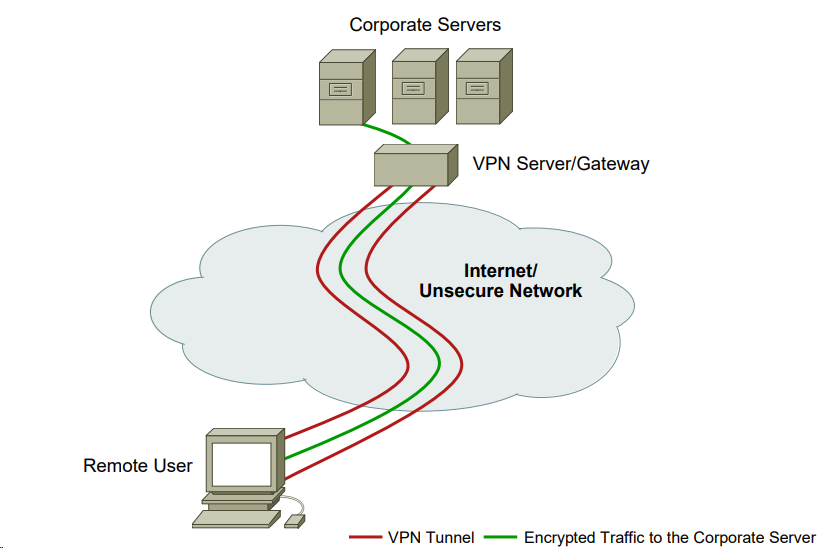
\includegraphics[width=.9\textwidth]{figures/VPNdemo}
	\caption{Ukážka typického VPN pripojenia}
	\label{vpndemo}
\end{figure}
% TODO: \usepackage{graphicx} required
\begin{figure}
	\centering
	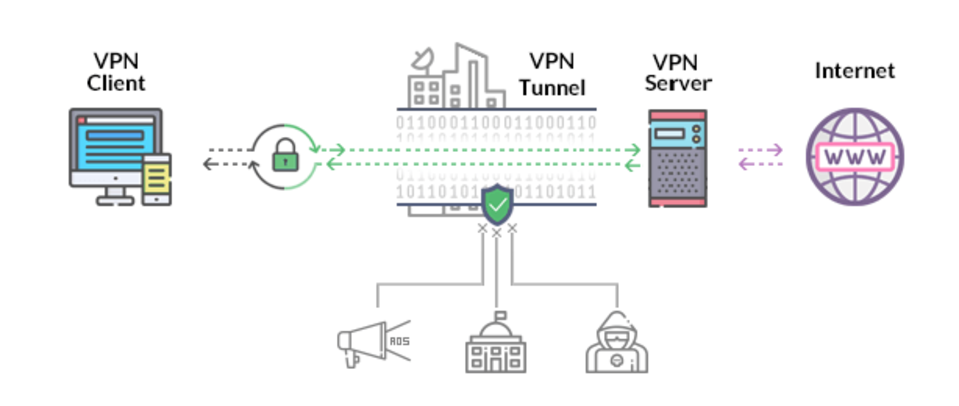
\includegraphics[width=0.7\linewidth]{figures/vpn_fancy}
	\caption{vpn fancy obrazok}
	\label{vpnfancy}
\end{figure}
\section{Výhody a nevýhody VPN sieti}
neviem ci to bude treba na samostatnu podkapitolu
mozno len doplnit informacie do textu 
\section{Klasifikácia VPN sietí}
V súčasnosti má čitateľ k dispozícií veľa rôznych internetových zdrojov o problematike VPN. Uvedené sú rôzne možnosti klasifikácie VPN siete. V rámci tejto práce klasifikujeme VPN siete podľa logickej topológie, použitých protokolov a vrstiev, na ktorých sú postupy aplikované. Obsahom tejto podkapitoly je rozdelenie a opis jednotlivých typov VPN sieti.
\subsection{Rozdelenie VPN sieti podľa logickej topológie}
 Podľa topológie, v ktorej VPN spojenie prebieha rozdeľujeme VPN do 3 kategórií: 
\begin{itemize}
	\item \textbf{VPN rovný s rovným} -- \textit{z ang. Peer to Peer VPN},
	\item \textbf{VPN klient a server} -- \textit{z ang. Client to Server VPN}, 
	\item \textbf{VPN sieť so sieťou} -- \textit{z ang. Site to Site VPN}.
\end{itemize}

\subsubsection{VPN rovný s rovným}
Uvedený spôsob vytvára zabezpečený tunel medzi dvoma rovnocennými uzlami, resp. zariadeniami\footnote{z ang. \textit{peers}}, ktorý spoločne komunikujú cez verejnú sieť. Medzi zariadeniami je vytvorený tunel. Každý koniec má priradenú svoju IP adresu. Z uvedeného modelu vyplýva aj následná limitácia. VPN tunel vznikne iba medzi dvoma komunikujúcimi zariadeniami. Z toho dôvodu nie je toto použitie časté. Na obrázku \ref{p2p} je znázornený uvedený typ VPN spojenia. 
\begin{figure}[!ht]
	\centering
	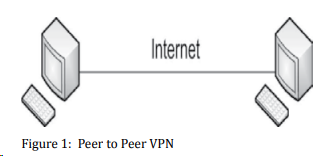
\includegraphics[width=.7\textwidth]{figures/p2p}
	\caption{}
	\label{p2p}
\end{figure}
 
\subsubsection{VPN Klient a Server}
Tento typ spojenia pozostáva z pripojenia medzi nerovnocennými dvoma alebo viacerými zariadeniami. Najjednoduchší model musí pozostávať z jedného VPN servera a VPN klienta. Princíp spočíva vo vytvorení zabezpečeného tunela, ktorý je použitý na prenos dát medzi uvedenými zariadeniami. Zároveň je však možné vytvoriť $1:N$ takýchto spojení. $N$ reprezentuje počet VPN klientov, resp. prepojení, ktorý VPN Server dokáže nadviazať. Tento parameter je závislý najmä od hardvérových prostriedkov daného servera.

Úloha Klienta spočíva v presmerovaní všetkej svojej sieťovej komunikácie cez zabezpečený tunel, ktorý vznikol medzi ním a Serverom. Tento úkon je najčastejšie realizovaný presmerovaním trafiky cez sieťovú bránu\footnote{z ang. \textit{GateWay}} (ďalej \acrshort{gw}). V danom \acrshort{os}, na ktorom VPN klient beží, je teda potrebné zmeniť IP adresu \acrshort{gw} na adresu VPN servera. Vďaka tomu nastane presmerovania komunikácie. Tento úkon je väčšinou realizovaný programovo pomocou aplikácií. Typicky nastolia spojenie medzi Klientom a Serverom. Následne upravia sieťové nastavenia systému. Spomenuté úkony sú vysoko závislé od \acrshort{os} a daného programovacieho jazyka, prostredníctvom ktorého sú úpravy realizované. 
Úloha Servera na druhej strane spočíva vo vytvorení možnosti pripojenia pre jedného alebo viacerých klientov. Následne Server zastupuje klientovu prítomnosť v danej sieti. Teda spracúva požiadavky Klienta a komunikuje s ostatnými zariadeniami. Komunikácia ďalej však už nie je zabezpečená pomocou šifrovania alebo tunelu. Tento fakt je znázornený na obrázku \ref{c2s}.   

\begin{figure}[!ht]
	\centering
	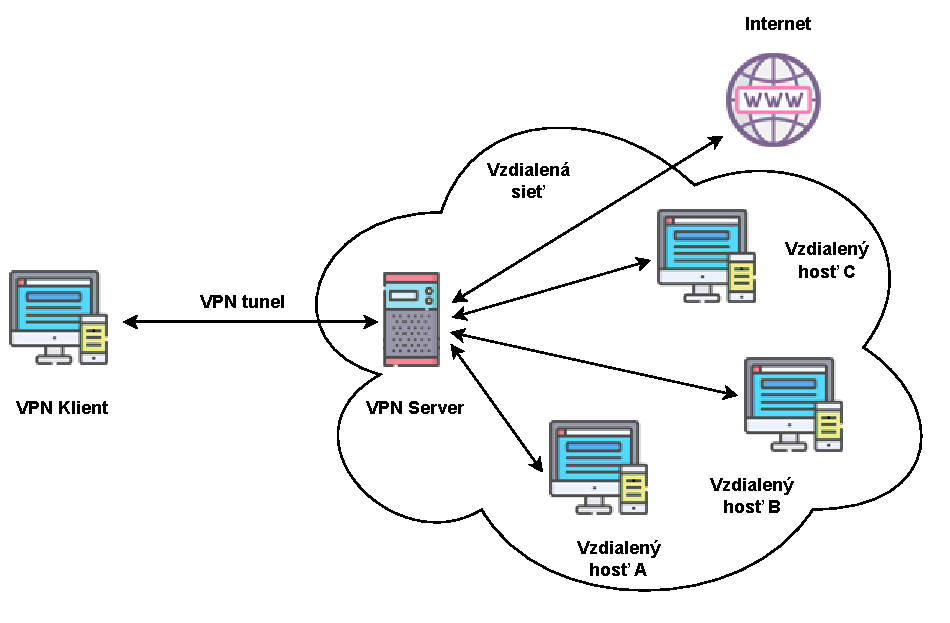
\includegraphics[width=.7\textwidth]{figures/c2s}
	\caption{potrebne prerobenie nech sa to nepodoba na 1.1 alebo vyhodit/upravit 1.1}
	\label{c2s}
\end{figure}
V súčasnosti je tento spôsob považovaný za najviac používaný v oblasti korporátneho sveta. VPN server slúži ako vstupná brána do internej siete. Vďaka tomu je možné sprístupniť zdroje pre používateľov z rôznych oblastí sveta. Používateľ sa taktiež môže stretnúť s pomenovaním model \textbf{uzol k sieti}, resp. z ang \textit{point-to-site}. Obidva pojmy sú správne a predstavujú rovnakú myšlienku zapojenia VPN.  
\subsubsection{Sieť so Sieťou VPN}
VPN model Sieť so Sieťou vytvára zabezpečený tunel medzi dvoma rôznymi sieťami naprieč verejnou sieťou. Model pozostáva z 2 zariadení -- VPN servera a VPN Koncentrátora\footnote{z ang. \textit{VPN Concentrator}}.

VPN Koncentrátor je typ sieťového zariadenia, ktoré poskytuje zabezpečené VPN spojenie a doručenie dát. Zvyčajne je to špecializovaný smerovač\footnote{z ang. \textit{router}}. Dokáže vytvárať veľké množstvo VPN tunelov. Používa sa na nastolenie VPN modelu sieť so sieťou. Funkcionalita koncentrátora pozostáva z: 
\begin{itemize}
	\item{nastolenie a konfiguráciu VPN tunela} -- z ang. \textit{Establish and Configure tunnels},
	\item{autentizáciu používateľa}-- z ang. \textit{Authenticate users},
	\item{priradenie IP adries používateľov k tunelom} -- z ang. \textit{Assign tunnel/IP addresses to users},
	\item{šifrovanie a dešifrovanie dát} -- z ang. \textit{Encrypt and Decrypt data},
	\item{zabezpečiť integritu doručenia} -- z ang. \textit{Ensure end-to-end delivery of data}.
\end{itemize}

Model Sieť so sieťou je používaný najmä pri spojení vedľajšej pobočky s hlavnou, ktoré sa nachádzajú na rozdielnych geografických lokalitách. Pomocou schémy \ref{sts} je znázronený tento model. 

 \begin{figure}[!ht]
 	\centering
 	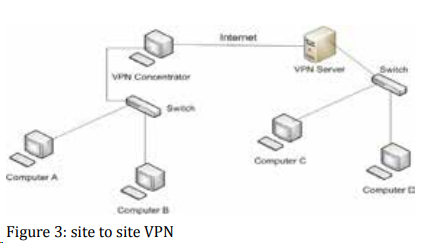
\includegraphics[width=.7\textwidth]{figures/sts}
 	\caption{rearanzovat}
 	\label{sts}
 \end{figure}
\subsection{Rozdelenie VPN sieti podľa použitých protokolov}      
\subsection{Rozdelenie VPN sieti podľa vrstiev TCP/IP referenčného modelu}\label{rm}
\subsubsection{Charakteristika referenčných modelov}
V rámci  podkapitoly \ref{rm} je potrebné pred samotnou klasifikáciou vysvetliť pojmy Referenčný model prepojenia otvorených systémov\footnote{z ang. \textit{Open Systems Interconnection reference model}} (ďalej \acrshort{osi}) a Model opisujúci balíky internetových protokolov, známy ako, \acrshort{tcpip} referenčný model.

Úlohou uvedených referenčných modelov je vizualizácia postupu spracovania dát od používateľa až k ich odoslaniu zo zariadenia\footnote{z ang. \textit{end-to-end data communication}}. Pojem spracovanie dát znamená opísanie toho ako dochádza v jednotlivých abstraktných vrstvách k pretransformovaniu používateľských dát na súbor jednotiek a núl, ktoré sú následne odoslané do iného zariadenia. 

\acrshort{osi} Model vznikol v skorších fázach evolúcie počítačových sietí. Vychádza skôr z teoretického než praktického prístupu. Pozostáva zo 7 abstraktných vrstiev:

\begin{itemize}
	\item{fyzická vrstva} -- vrstva 1 (ďalej L1), 
	\item{spojová vrstva} -- vrstva 2 (ďalej L2),
	\item{sieťová vrstva} -- vrstva 3 (ďalej L3),
	\item{transportná vrstva} -- vrstva 4 (ďalej L4),
	\item{relačná vrstva} -- vrstva 5 (ďalej L5),
	\item{prezenčná vrstva} -- vrstva 6 (ďalej L6),
	\item{aplikačná vrstva} -- vrstva 7 (ďalej L7).
\end{itemize}

Čím je väčšie číslo vrstvy tým bližšie sa dáta nachádzajú pri používateľovi. Vďaka uvedeným vlastnostiam je tento model vhodnejší pri začiatku štúdia spracovania sieťových dát v počítači. Viac informácií o problematike nájde čitateľ v \cite{osi}.

Na druhej strane \acrshort{tcpip} model vznikol z praktického prístupu. Hlavný rozdiel je v počte abstraktných vrstiev, ktorý je v prípade \acrshort{tcpip} zmenšený na 4 vrstvy \cite{tcpip}. 
TCP/IP model je zobrazený pomocou schémy \ref{tcpipprot}. V uvedenej schéme sú znázornené aj niektoré z protokolov, ktoré sa na jednotlivých vrstvách používajú.

\begin{figure}[!ht]
	\centering
	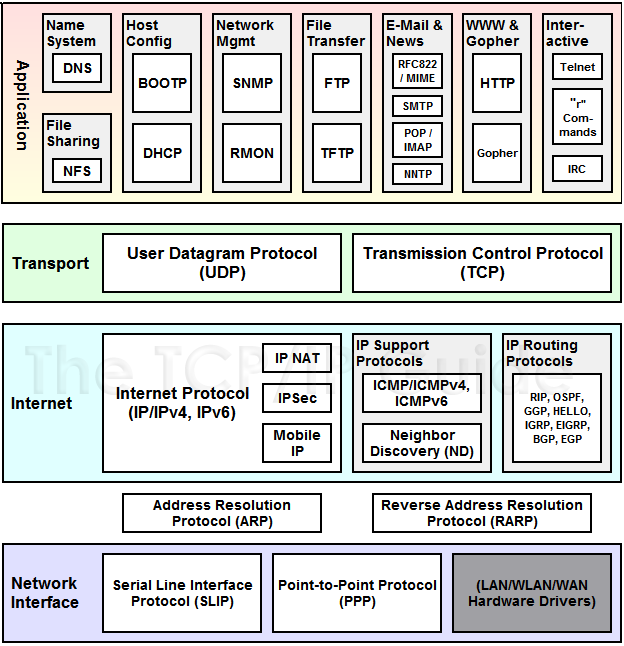
\includegraphics[width=0.9\textwidth]{figures/tcpipprot}
	\caption{Schéma TCP/IP modelu s niektorými protokolmi}
	\label{tcpipprot}
\end{figure}

\textbf{Aplikačná vrstva (L5-7)} zahŕňa protokoly používané väčšinou aplikácií na poskytovanie užívateľských služieb alebo výmenu aplikačných dát cez sieťové pripojenia, ktoré je vytvorené protokolmi na nižšej úrovni.  Spája vrstvy L5 až L7 OSI modelu. Príklady známych protokolov aplikačnej vrstvy sú \acrfull{http}, \acrfull{ftp}, \acrfull{smtp} a iné. Údaje, resp. dáta sú pri spracovaní kódované podľa L4 protokolov. Sú zapuzdrené do protokolových jednotiek transportnej vrstvy, tzv. \textbf{segmentov}.  

\textbf{Transportná vrstva (L4)} vytvára základné dátové kanály, ktoré aplikácie používajú na výmenu dát. Vrstva vytvára konektivitu medzi hostiteľmi, ktorá je nezávislá od siete, štruktúry užívateľských dát a smerovacích informácií. Konektivita na transportnej vrstve môže byť kategorizovaná ako orientovaná na spojenie, implementovaná v protokole \acrshort{tcp}, alebo \acrshort{udp} bez orientácie na spojenie. Uvedené protokoly sú stručne charakterizované nižšie, v tejto podkapitole. 

Protokoly v tejto vrstve zabezpečujú:
\begin{itemize}
	\item{riadenie chýb} -- z ang. \textit{error control} \cite{ec},
	\item{segmentáciu dát} -- z ang. \textit{segmentation} \cite{sd},
	\item{riadenie toku dát} -- z ang. \textit{flow control} \cite{fc},
	\item{riadenie preťaženia} -- z ang. \textit{congestion control} \cite{cc},
	\item{adresovanie aplikácií} -- z ang. \textit{application addressing} \cite{aa}.
\end{itemize}
Výstupom transportnej vrstvy sú segmenty, ktoré sú spracované v ďalšej vrstve referenčného modelu. 

\textbf{Internetová, resp. Sieťová vrstva (L3)} je zodpovedná za odosielanie paketov cez jednu alebo viac sietí. S touto funkcionalitou internetová vrstva umožňuje sieťovanie, prepojenie rôznych IP sietí a v podstate vytvára internet. Z L4 segmentov tvorí pakety, tak že pridá informácie potrebné na ďalšie smerovanie. 

\textbf{Linková vrstva (L2)} sa používa na presun paketov medzi rozhraniami internetovej vrstvy dvoch rôznych hostiteľov na rovnakom linku. Procesy vysielania a prijímania paketov na linke je možné konfigurovať. Zariadenia nazývané prepínače \footnote{z ang. \textit{Switch}}, vykonávajú rámcovania\footnote{z ang. \textit{frame}}. Pripravujú pakety z L3 vrstvy na prenos pridaním ďalších informácií. Týmto úkonom vzniknú rámce. Tie sa prenášajú do fyzickej vrstvy a cez prenosové médium až k hostiteľovi. Fyzická vrstva predstavuje prvok, cez ktoré sú dáta prenášane. Napríklad optický a ethernetový kábel. 

Vyššie uvedené procesy prípravy dát sú znázornené pomocou schémy \ref{p1} a \ref{p2}.
% TODO: \usepackage{graphicx} required
\begin{figure}
	\centering
	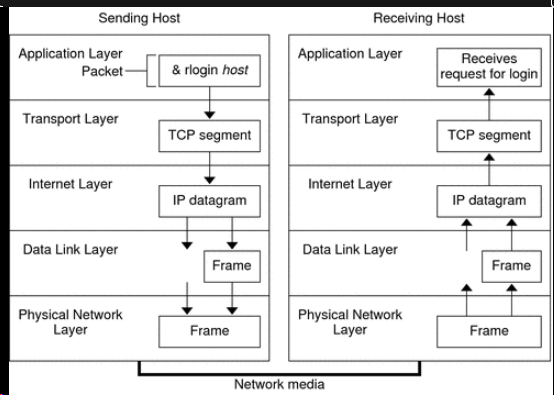
\includegraphics[width=0.7\linewidth]{figures/prenos1z2}
	\caption{spoj tento obrazok s nasledujucim do jedneho}
	\label{p1}
\end{figure}
% TODO: \usepackage{graphicx} required
\begin{figure}
	\centering
	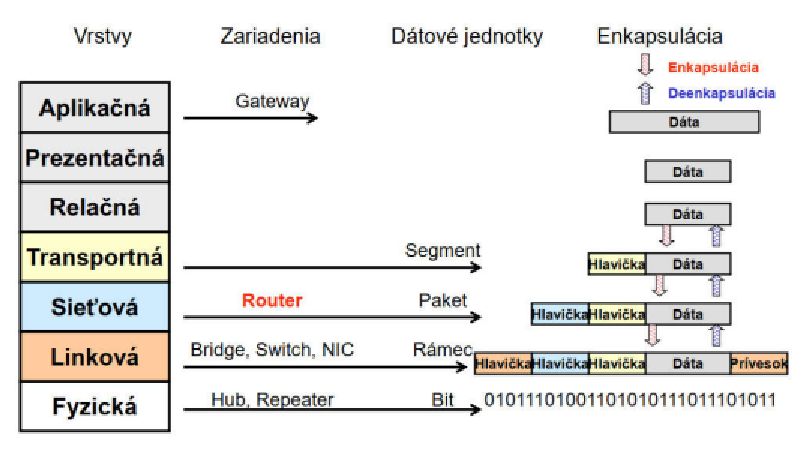
\includegraphics[width=0.7\linewidth]{figures/prenos2z2}
	\caption{spoj tento obrazok s predchadzajucim do jedneho}
	\label{p2}
\end{figure}

\textbf{Protokol riadenia prenosu} (z ang. \textit{Transmission Control Protocol}, ďalej \acrshort{tcp}) je komunikačný protokol orientovaný na nadviazanie a udržanie sieťového spojenia medzi zariadeniami. Môže byť použitý pri úlohe príjímateľa aj odosielateľa (z ang. \textit{full-duplex}). Úlohou je spoľahlivý prenos dát medzi komunikantmi. Odoslanie a príjem dát je v rovnakom poradí. Protokol zároveň obsahuje mechanizmy na kontrolu výskytu chýb. Svoj názov má podľa dvoch najdôležitejších protokolov:
\begin{itemize}
	\item{Protokol Riadenia Prenosu} -- z ang. \textit{\acrlong{tcp}},
	\item{Internet Protokol} -- z ang. \textit{\acrlong{ip}}. 
\end{itemize}

Na začiatku 21. storočia je 95\% paketov používaných na internete TCP. Bežné aplikácie používajúce TCP sú webové (HTTP/HTTPS protokoly), slúžiace na e-mailovú komunikáciu (SMTP/POP3/IMAP) a prenos súborov (z ang. \textit{File Transfer Protocol -- \acrshort{ftp}}). Minimálna dĺžka hlavičky TCP je 20 bajtov a maximálna dĺžka 60 bajtov. Po pridaní údajov TCP hlavičky k prenášaným dátam, vzniká tzv. \textit{segment}.

V súčasnosti je možne TCP protokol implementovať softvérovo aj hardvérovo. Pri prvom z uvedených je problémom závislosť na OS a následne aj vysoká vyťaženosť procesora pri príprave a spracovaní dát. Pri hardvérovom riešení je výhodou optimalizácia a implementácia bez potreby dodatočnej úpravy OS. Hardvérové implementácie sa realizujú pomocou koprocesorov umiestnených vo vnútri procesora. Následkom toho môžeme dnes bežne pozorovať umiestnenie spomenutých zariadení na našich zariadeniach.

Podrobnejšie informácie o TCP protokole je možné nájsť na \cite{tcp2}. V uvedenej publikácií sa nachádza opis TCP hlavičky, metódy nadviazania a ukončenia spojenia. Obdobne je spomenuté ako dochádza k prenosu dát pomocou sekvenčných čísel. Ak má používateľ nejasnosti v fungovaní TCP protokolu, odporúča sa danú publikáciu prečítať.

\textbf{Používateľský datagramový protokol} (z ang. \textit{User Datagram Protocol}, ďalej \acrshort{udp}) je jedným zo základných komunikačných \acrshort{ip} protokolov. Používa sa na odosielanie správ iným hostiteľom v sieti. Správy sú prenášané ako datagramy v paketoch. \acrshort{udp} nevyžaduje predchádzajúcu komunikáciu na nastavenie komunikačných kanálov alebo dátových ciest. Používa jednoduchý komunikačný model bez spojenia s minimom protokolových mechanizmov. Poskytuje kontrolné súčty pre integritu údajov a čísla portov na adresovanie rôznych funkcií v zdroji a cieli datagramu. 

Narozdiel od \acrshort{tcp}) neposkytuje žiadnu záruka doručenia správy alebo duplicitnej ochrany. 
\acrshort{udp}) je vhodný na účely, kde kontrola a oprava chýb buď nie sú potrebné, alebo sa vykonávajú v aplikácii. Aplikácie citlivé na čas často používajú UDP, pretože zahadzovanie paketov je vhodnejšie ako čakanie na pakety oneskorené v dôsledku opätovného prenosu. Príklad použitia môžu byť streamovacie služby. 
Podrobnejšie informácie o \acrshort{udp}) protokole nájde čitateľ v \cite{udp}.

\subsection{Klasifikácie VPN sieti}

\cite{divvpn}, \cite{ciscovpn}
https://www.vpnmentor.com/blog/different-types-of-vpns-and-when-to-use-them/
https://www.top10vpn.com/what-is-a-vpn/vpn-types/
%https://en.wikipedia.org/wiki/Virtual_private_network
%https://csrc.nist.gov/glossary/term/virtual_private_network
https://www.auvik.com/franklyit/blog/vpn-types/
https://www.geeksforgeeks.org/types-of-virtual-private-network-vpn-and-its-protocols/?ref=rp
https://www.geeksforgeeks.org/difference-between-site-to-site-vpn-and-remote-access-vpn/?ref=rp


\section{Kryptografické zabezpečenie protokolov}
TCP protokol sam o sebe nezabezpečí dáta, ku ktorým sa pridáva TCP hlavička. Dôsledkom toho vznikli viacere protokoly slúžiace na autentizované šifrovanie dát. Najznámejší je protokol zabezpečenia prenosu -- \acrshort{tls} a IPSec.
\subsection{Transport Layer Security -- TLS}
Zabezpečenie dát bolo prvotne vykonávané pomocou protokolu \textit{Secure Sockets Layer} -- \acrshort{ssl}. Tento spôsob používa certifikáty na odšifrovanie dát. SSL malo od svojho vytvorenia dlhý vývoj, ktorý smeroval až k doteraz najpoužívanejšiemu TLS vo verzii 1.3. Inými slovami, TLS protokol je nástupca SSL pričom obsahuje rôzne úpravy a vylepšenia najmä z hľadiska rýchlosti. Zároveň sa v dnešnej dobe neodporúča používanie SSL protokolu. Dôsledkom optimalizácií je, že klienta komunikujúci so serverom cez HTTPS protokol s TLS 1.3 je rýchlejší ako v prípade použitia nešifrovaného HTTP variantu. 

TLS pracuje niekde na pomedzi aplikačnej a transportnej vrstvy. Spôsob spracovania dát je zobrazený pomocou schémy \ref{ssl} s SSL operáciami, prebratej z \cite{biks}. 
\begin{figure}[!ht]
	\centering
	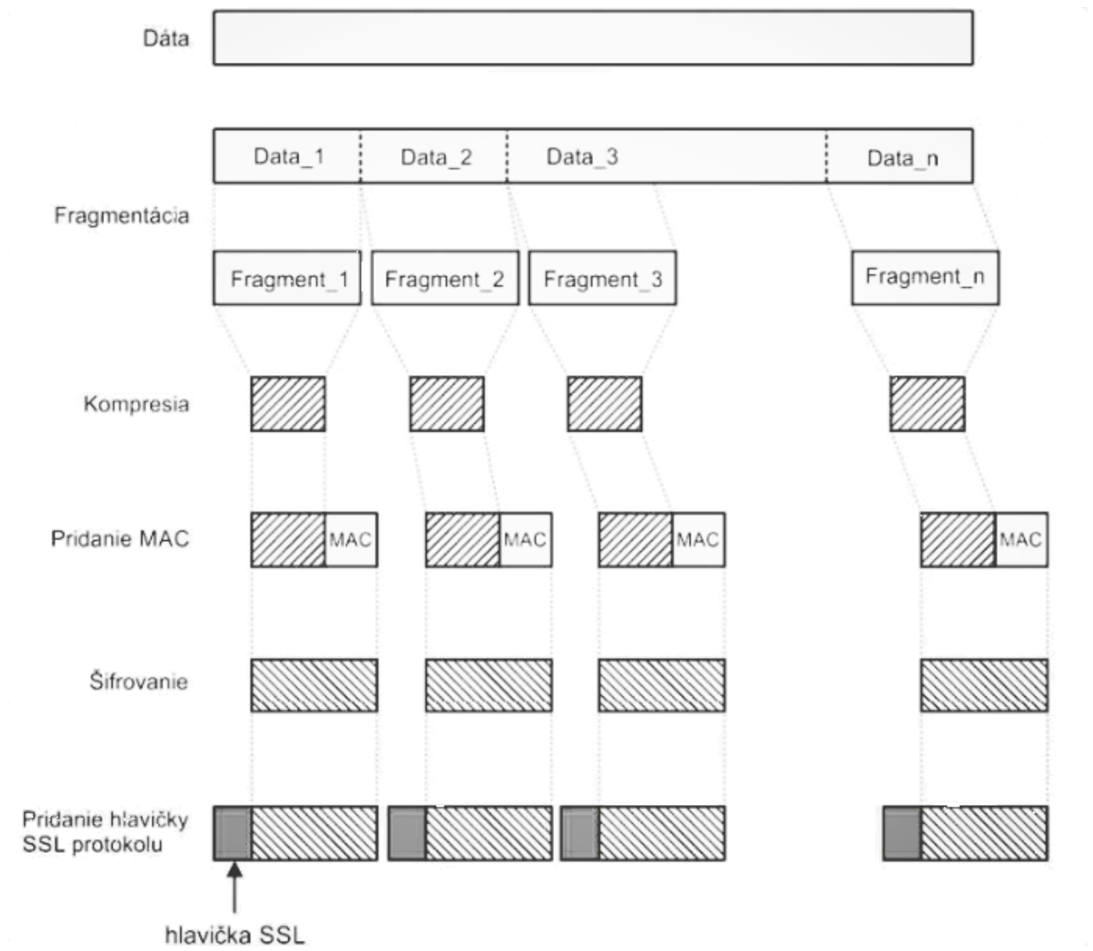
\includegraphics[width=0.7\linewidth]{figures/ssl}
	\caption{Prehľad operácií v SSL protokole}
	\label{ssl}
\end{figure}

Viac informácií o TLS protokole, jednotlivých verziách a optimalizáciách je možné nájsť na \cite{tls}. 

\subsection{Internet Protocol Security  -- IPSec}
Ochrana medzi transportnou a sietovou vrstvou TCL/IP.
Nabudúce. \cite{biks}
\chapter{Kryptografia vo VPN}\label{krypto}
Cieľom kryptografických blokov je utajiť správu pri jej ceste z bodu A do B. Teda od odosielateľa (tvorcu) správy, až k jej prijímateľovi. Dôsledkom tohto úkonu dochádza k zabezpečeniu 3 hlavných úloh kryptografie:
\begin{itemize}
	\item \textbf{ochrana osobných údajov} (dôvernosť) -- z ang. \textit{Data Privacy}, 
	\item \textbf{autenticita údajov} (prišla z miesta, kde sa uvádza)  -- z ang. \textit{Data Authenticity},
	\item \textbf{integrita údajov} (nebolia upravená počas prenosu)  -- z ang. \textit{Data Integrity}.
\end{itemize}

 Prvý z uvedených bodov je najčastejšie žiadaným a známym cieľom. Odosielateľ správy zašifruje jej obsah pomocou použitia niektorého z šifrovacích algoritmov, kryptografického kľúča a následne správu odošle. Na druhej strane, prijímateľ, musí použiť komplementárny dešifrovací algoritmus s prislúchajúcim kľúčom. Ktokoľvek kto sa dostane medzi týchto komunikantov, k takto preposielanej správe, z nej nedokáže obsahovo nič zistiť, v istom časovom období. 
 
 Dôsledkom týchto faktov je jasné, že komunikanti musia mať jasne definovaný použitý algoritmus. Zároveň je nutné aby došlo k výmene kryptografických kľúčov, ktoré sú pri šifrovaní a dešifrovaní aplikované. Tým sa zabezpečí aj druhá úloha -- Autenticita dát, pretože potrebné informácie budú mať len komunikanti. 
 
 V kryptografických blokoch sú taktiež aplikované algoritmy na overenie integrity správ. Ich úlohou je potvrdiť, že do obsahu správy nebolo, počas jej transportu medzi komunikantmi, nič pridané, resp. ubrané.
 
 V súčasnosti má používateľ možnosť vybrať si zo širokej ponuky kryptografických algoritmov. Medzi najznámejší patrí \acrshort{aes} \cite{aes}, ktorý je aktuálne používaný ako štandardný kryptografický algoritmus. Detailný opis jednotlivých blokov a postupov použitých v AES-e, je obsahom rôznych vydaní. Viac informácií o problematike nájde čitateľ v \cite{levicky}, ktorá obsahuje okrem opisu AES-u aj doležité informácie, týkajúce sa kryptografických základov.

V rámci tejto práce sme sa rozhodli opísať, v súčásnosti menej známe, algoritmy: 
\begin{itemize}
	\item XOODOO \cite{tkecak}
	\item Gimli \cite{gimli}
	\item Simpira384 \cite{simpira}
\end{itemize}  
Uvedené permutácie sú použité ako kryptografické primitívum a pri následnej tvorbe ďalších kryptografickych blokov. 

\section{Kryptografický algoritmus XOODOO a variácie} 
XOODOO je sada 384-bitových kryptografických permutácií parametrizovaných počtom kôl. Funkcia kola/rundy\footnote{z ang. \textit{round}} funguje na 12 slovách\footnote{z ang. \textit{words}} po 32 bitoch. Vďaka tomu je efektívna aj na menej výkonných procesoroch nižšej triedy. Vytvoril ju tím Keccak, ktorý stojí za viacerými úspešnými kryptografickými algoritmami. Napríklad hashovacie funkcie z rodiny SHA-3 a iné -- \cite{kecsup}. XOODOO algoritmus vznikol po vytvorení tzv. Kravatte autentizačno-šifrovacieho algoritmu \cite{kravatte}, založené na Keccak-p permutácií \cite{keccakp}. Ten sa ukázal ako dostatočne rýchly na širokom spektre platforiem. Avšak nezapadá do kategórie tzv. ľahkej kryptografie \footnote{z ang. \textit{lightweight cryptography}}.

Tím Keccak vypracoval nové riešenie. Ním bol port medzi ich prvotným Keccak-p dizajnom a Gimli-ho \cite{bernstein2017gimli} permutačným algoritmom. Vo výsledku autori zlúčili lepšie realizované prvky z oboch algoritmov do jedného celku. Primárny problém samotnej Gimli permutácie bol v slabom prejave zmeny výstupu po malých zmenách vo vstupnej správe. Táto vlastnosť sa v kryptografii označuje pomocou anglického pojmu, tzv. \textit{propagation properties}\footnote{Cieľom je aby aj zmena jedného bitu na vstupe, ovplyvnila čo najviac bitov vo výstupe -- tzv. \textit{Lavínový efekt}.}. Novo-vzniknuté riešenie autori pomenovali XOODOO. Na základe rôznych variácií tohto kryptografického primitíva sa im následne podarilo vytvoriť sadu vysoko efektívnych kryptografických funkcií. 
Medzi sady, ktorých jadro tvorí XOODOO, patrí Xoodyak a Xoofff. Xoofff pozostáva zo zlúčenia Farfalle konštrukcie \cite{farfalle} so XOODOO permutáciou. 

Xoodyak ma narozdiel od Xoofff duplexovú konštrukciu \cite{duplex}. Vo výsledku máme ľahko prenosnú, všestrannú, kryptografickú knižnicu. Je vhodná do výkonovo obmedzených prostredí. Môže sa použiť pre väčšinu kryptografických funkcií, ktoré používajú symetrický kľúč. Napríklad hashovanie, šifrovanie, výpočet MAC alebo autentizované šifrovanie. O kvalite riešenia napovedá aj fakt, že sada Xoodyak je jedným z 10 finalistov v oblasti ľahkej kryptografie NIST štandardizačného procesu.
V rámci tejto kapitoly opíšeme kryptografické primitívum XOODOO a následne balík Xoodyak. Informácie o téme boli čerpané z týchto zdrojov: \cite{tkecak}, \cite{xd}, \cite{xcb}, \cite{xoodoocb}, \cite{xdupdate},\cite{xdr1}.
\subsection{XOODOO permutácia}
XOODOO je rodina permutácií, ktorá je definovaná počtom rúnd. Má klasickú iteračnú štruktúru. Teda opakovateľne sa vola rundová funkcia s aktuálnym stavom. Pre pochopenie operácií je nutné pochopiť určité označenie použité v algoritme.

Stav -- \textbf{state}, pozostáva z 3 rovnako veľkých horizontálnych rovín -- \textbf{planes}. Každá z týchto rovín obsahuje štyri paralelne 32-bitové pruhy -- \textbf{lanes}. Okrem tejto charakteristiky je možné opísať stav ako množinu 128 stĺpcov -- \textbf{columns}, pričom jeden stĺpec obsahuje 3 bity v každej rovine. Stav je teda tvorený zo stĺpcov usporiadaných v poli o rozmere 4x32. Posledná položka na opis stavu sú tzv. listy -- \textbf{sheets}. List sa skladá z 3 na sebe uložených pruhov. Uvedené pojmy sú znázornené pomocou schémy \ref{xoodooterm}, ktorá bola prebraná z \cite{xcb}.

\begin{figure}[!h]
	\centering
	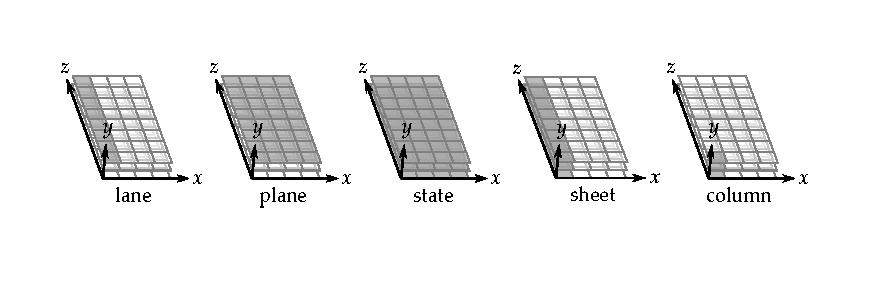
\includegraphics[width=1\textwidth]{figures/xoodooTerminology}
	\caption{Grafické znázornenie terminológie v XOODOO}
	\label{xoodooterm}
\end{figure}

Roviny majú index $y$. $y=0$ zodpovedá spodnej rovine a vrchná rovina $y=2$. Bit je označený s indexom $z$ vrámci množiny pruhov. List ich označujeme pomocou indexu $x$. Takže pozícia pruhu v stave je definovaná pomocou dvoch súradníc $(x,y)$. Konkrétny bit je možné v stave následne reprezentovať pomocou trojice súradníc $(x,y,z)$. Pri učení stĺpca sú potrebné 2 súradnice $(x,z)$. Pred spustením samotného algoritmu musí používateľ vykonať mapovanie 384-bitovej správy voči horizontálnym rovinám. Tento úkon sa realizuje pomocou vzorca \ref{index}.

\begin{equation}\label{index}
	i=z+32(x+4y)
\end{equation}

Rundová funkcia pozostáva z 5 krokov:
\begin{enumerate}
	\item miešanie vrstvy (z ang. \textit{a mixing layer $\theta$}), 
	\item posun rovín (z ang. \textit{a plane shifting $\rho_{west}$}), 
	\item pridanie rundových konštánt (z ang. \textit{the addition of round constants $\iota$}),
	\item nelineárna vrstva (z ang. \textit{a non-linear layer $\chi$}),
	\item posun rovín (z ang. \textit{an another plane shifting $\rho_{east}$}).
\end{enumerate}
Opis jednotlivých krokov je znázornený pomocou schémy \ref{xoodooalgo}, ktorá je prebratá z \cite{xcb}. Schéma opisuje jednotlivé kroky algoritmu vrátane rundových konštánt. 

  \begin{figure}[!h]
  	\centering
  	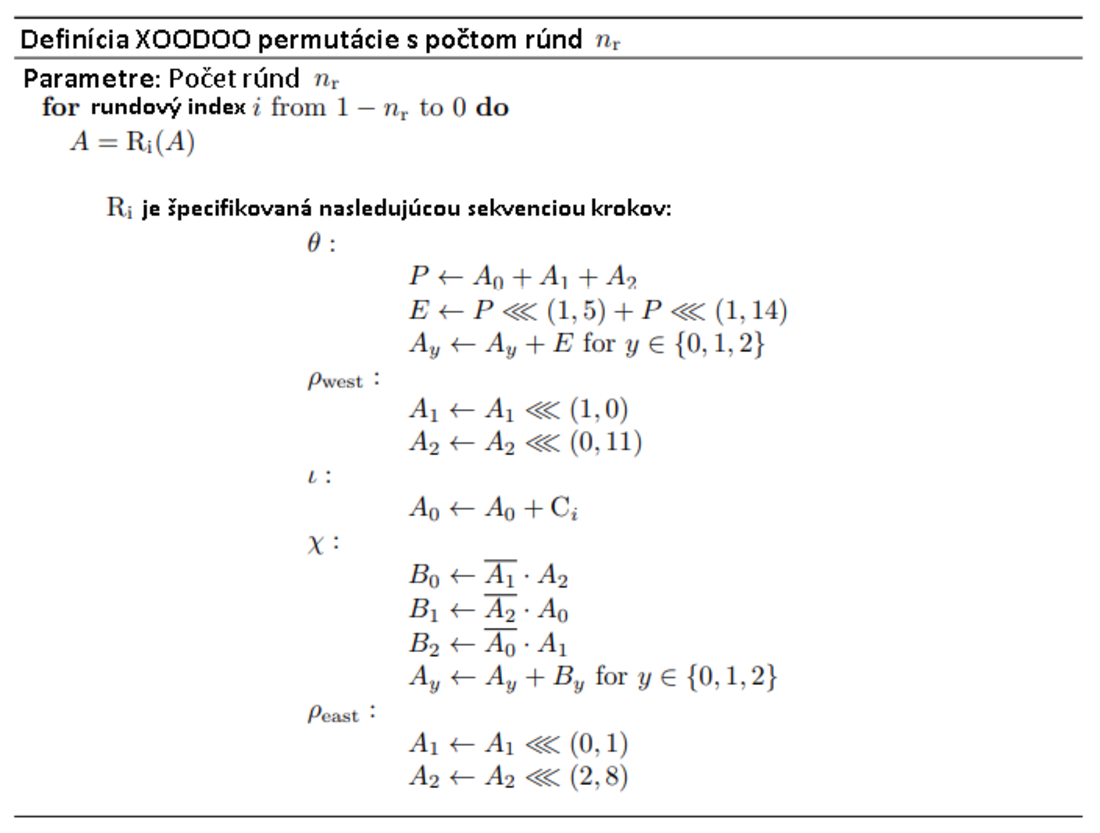
\includegraphics[width=1.1\textwidth]{figures/xoodooalgo}
  	\caption{}
  	\label{xoodooalgo}
  \end{figure}

\subsection{Xoodyak} 
Xoodyak možno považovať za všestranný kryptografický nástroj. Je vhodný pre väčšinu operácií využívajúcich symetrický kľúč. Napríklad generovanie pseudonáhodných bitov, autentizáciu, šifrovanie a iné. Tím Keccak použil pri návrhu duplexnú konštrukciu. Konkrétne variant s plným stavom a využitím kľúča. Tento dizajn označujeme ako \acrfull{fskd}. Viac o tejto konštrukcii si čitateľ môže prečítať v \cite{duplex}.
Operačný režim, v ktorom Xoodyak pracuje sa nazýva Cyklista -- z ang. \textit{Cyclist}. Tento názov získal ako opozitum k pomenovaniu režimu Motorista, ktorý je možné nájsť v Keyak schéme \cite{keyak}. Narozdiel od uvedeného balíka Keyak, nie je Xoodyak limitovaný len na autentizované šifrovanie. Je jednoduchší hlavne kvôli tomu že neobsahuje paralelné varianty.

\subsubsection{Režim Cyklista}\label{cyklista}
Režim Cyklista funguje na princípe kryptografických permutácií $f$, teda zmeny usporiadania bitov za pomoci tajného kľúča a matematických operácií. Parametrami sú veľkosti blokov $R_{hash}$, $R_{kin}$, $R_{kout}$ a veľkosť račety, resp. západky\footnote{z ang. \textit{the ratchet size}} \cite{ratchet} $\ell_{ratchet}$. Uvedený pojem sa v kryptografii používa vo forme obrazného pomenovania. Cieľom je poukázať na jednoduchý pohyb vpred, ale s ťažkým, resp. zložitejším pohybom naspäť. Dôležité je, že uvedený scenár je vyvolaný zámerným dizajnom. Šírka permutácie $b'$ je definovaná pomocou vzorca \ref{index2}. Všetky uvedené parametre sú v bajtoch. Pre označenie prázdneho slova budeme používať $\epsilon$.
\begin{equation}\label{index2}
	max(R_{hash}, R_{kin}, R_{kout}) + 2 \leq b'
\end{equation} 

Cyklista operuje v dvoch režimoch -- \textbf{hašovací a kľúčový}\footnote{z ang. \textit{hash and keyed mode}.}. 
Inicializácia prebieha pomocou príkazu \lstinline|CYCLIST(K,id,counter)|. Ak sa parameter $K$ rovná prázdnemu slovu $\epsilon$, tak potom nastane spustenie v hašovacom režime. Aktuálne nie je do implementácie zakomponovaná možnosť zmeny režimu po inicializácií. Vývojári však túto vlastnosť nevylúčili pre prípadné aktualizácie balíka.  


Dostupné funkcie závisia od režimu, v ktorom sa  Cyklista spúšťa. Medzi ne patria \lstinline|ABSORB()| a \lstinline|SQUEEZE()|. Možno ich volať v oboch režimoch, zatiaľ čo funkcie \lstinline|ENCRYPT()|, \lstinline|DECRYPT()|, \lstinline|SQUEEZEKEY()| a \lstinline|RATCHET()| sú dostupné len pre kľúčový režim. Účel každej funkcie je nasledujúci:
\begin{itemize}
	\item \lstinline|ABSORB(X)| absorbuje vstupný reťazec X,
	\item C $\gets$ \lstinline|ENCRYPT(P)| zašifruje P do C a absorbuje P,
	\item P $\gets$ \lstinline|DECRYPT(C)| dešifruje C do P a absorbuje P,
	\item Y $\gets$	\lstinline|SQUEEZE($\ell$)|  vytvára $\ell$-bajtový výstup, ktorý závisí od doteraz absorbovaných dát,
	\item Y $\gets$	\lstinline|SQUEEZEKEY($\ell$)| funguje ako \lstinline|SQUEEZE($\ell$)|, ale používa sa za účelom generovania odvodeného kľúča, 		\\ell nefunguje v listings pckg
	\item \lstinline|RATCHET()| transformuje stav na nevratný tak, aby sa zabezpečila dopredná bezpečnosť\footnote{z ang. \textit{Forward secrecy}} \cite{fsec}. 
\end{itemize}

Stav bude závisieť od postupnosti volaní funkcií a od jeho vstupných reťazcov. Presnejšie povedané, zámerom je, že akýkoľvek výstup závisí od postupnosti všetkých vstupných reťazcov a volaní, tak že akékoľvek dva nasledujúce výstupné reťazce budú výstupom rôznych domén. Napríklad volanie \lstinline|ABSORB(X)| znamená, že výstup bude závisieť od reťazca $X$. Na druhej strane \lstinline|ABSORB()| vo funkcii \lstinline|ENCRYPT(P)| vytvorí výstup závislý aj od $P$ z funkcie šifrovania. Okrem uvedených závislostí ovplyvňujú výstup aj iné dizajnové riešenia. Príkladom je minimalizácia pamäťovej stopy. Vo výsledku teda výstup závisí od počtu predchádzajúcich volaní funkcie \lstinline|SQUEEZE()| a predtým spracovaných textov pomocou funkcií \lstinline|ENCRYPT()| a \lstinline|DECRYPT()|. Viac informácií o režime je dostupných v kapitole 7.2, publikácie \cite{xcb}. 

\subsubsection{Definícia a bezpečnosť}
Xoodyak je definovaný pomocou operatívneho režimu Cyklista nasledovne:
\begin{equation}
	CYCLIST[f,R_{hash},R_{kin},R_{kout},\ell_{ratchet}]
\end{equation} 
Kde jednotlivé parametre majú veľkosti:
\begin{enumerate}
	\item $f$ -- permutácia XOODOO so šírkou 48 bajtov (384 bitov),
	\item $R_{hash}$ -- 16 bajtov,
	\item $R_{kin}$ -- 44 bajtov,
	\item $R_{kout}$ -- 24 bajtov,
	\item $\ell_{ratchet}$ -- 16 bajtov.  
\end{enumerate}
Takto definované parametre algoritmu dokážu poskytnúť 128-bitovú bezpečnosť v oboch režimoch Cyklistu. Samozrejmosťou je, že v prípade kľúčového režimu, musí byť veľkosť kľúča rovná alebo väčšia ako 128 bitov. Viac informácií o kryptografickej bezpečnosti algoritmov je možné nájsť v \cite{sec}.

Viac informácií o bezpečnosti Xoodyak-a je možné nájsť v \cite{xcb, 7.3}, odkiaľ boli informácie čerpané.

\subsection{Možnosti použitia Xoodyak algoritmu}
Obsahom tejto podkapitoly sú uvedené postupy ako a za akých okolností je daný balík možné použiť. 
\subsubsection{Použitie hašovacieho režimu}
Xoodyak sa dá aplikovať ako hašovacia funkcia.
\subsubsection{Použitie kľúčového režimu}
\section{Kryptografický algoritmus Gimli} 
\section{Kryptografický algoritmus Simpira384} 
